\section[Windows Internals]{Windows Internals}

To understand memory forensics on Windows, knowledge about Windows Internals is necessary, from memory model to some kernel design. In this section we will give the reader some technical details on Windows' design.

\subsection[Memory model]{Memory model}

We start by exploring the Windows memory model, and more importantly the Windows kernel memory model. Windows by default uses page size of 4KB, the virtual address space for each process is 2GB for the 32-bit version and 8TB for the 64-bit version. The system address space is 2GB for the 32-bit version and 248TB for the 64-bit version. For every processes, when run, can see both its own address space and the system space, but access to the system space is restricted. A typical 32-bit process can have a 2GB space for itself and a 2GB space of the system, makes a total virtual memory space 4GB. The system space, refer to as the kernel space, contains the OS kernel objects and the currently running drivers and kernel application. The kernel space uses \textit{pools} to manage objects allocation and deallocation. Windows has two types of pool, one that is \textit{pagable}, can swap out to disk, called \textit{paged pool} and the other \textit{non-paged pool}. The size of these two types of pool on Windows 10 can be reference through the Table~\ref{tab:poolsize} \cite{memorylimit}. Because many parts of the OS is not used often, Windows can swap those pages out to make more space. However, some information will always remained in the non-paged pools.

\begin{center}
\begin{table}[h]
\begin{tabular}{l p{5cm} p{5cm} }
Pool Type & Limit on 32-bit & Limit on 64-bit \\ \hline
Paged Pool & 384 GB or system commit limit, whichever is smaller & 384 GB or system commit limit, whichever is smaller \\
Non-paged Pool & 75\% of RAM or 2 GB, whichever is smaller. & RAM or 128 GB, whichever is smaller (address space is limited to 2 x RAM) \\
\end{tabular}
\caption{Pool size on Windows 10}
\label{tab:poolsize}
\end{table}
\end{center}

The memory pool is a bitmap\footnote{An array of bits}. Windows will return the pointer and size when asked for space in the pool (chunk). Windows keeps track of chunks in the pool. At first, there is only one chunk (the pool itself). When the user asks for space, Windows will split the chunk into two, one for the user and one left unused, Windows will keep spliting the unused space in pool and return to the user for any allocation requested. Upon deallocation, Windows will merge unused chunks into one. Consider the code in Listing~\ref{lst:basicpool} for a basic example of pool allocation.

% TODO: Picture

Each chunk will have a \texttt{POOL\_HEADER} field on top to denote the content of the chunk. \texttt{POOL\_HEADER} has a size field (\texttt{BlockSize}), a previous size field (\texttt{PreviousBlockSize}), and a tag (\texttt{POOL\_TAG}). Tag is a four-byte character that Windows and Driver writer use to denote the data stored in the chunk. In Table~\ref{tab:pooltag}, we listed some typical structure with its tag.
\lstinputlisting[language=C,caption={Basic Pool Algorithm},label={lst:basicpool},basicstyle=\linespread{0.8}]{code/basic_pool.cpp}

\begin{center}
\begin{table}[h]
\begin{tabular}{lll}
Structure     & Structure Name   & Pool Tag \\ \hline
Driver Object & \_DRIVER\_OBJECT & Driv     \\
File Object   & \_FILE\_OBJECT   & File     \\
Process       & \_EPROCESS       & Proc     \\
TCP endpoint  &                  & TcpE     \\
TCP listener  &                  & TcpL     \\
Thread        & \_ETHREAD        & Thre     \\
UDP endpoint  &                  & UdpA     \\
\end{tabular}
\caption{Some pool tag and corresponding structure}
\label{tab:pooltag}
\end{table}
\end{center}

\subsection[EPROCESS and ETHREAD]{EPROCESS and ETHREAD}

Windows has a special structure that contains a process information called \texttt{\_EPROCESS}. This structure is created every time when a new process spawns and located inside a non-paged pool with tag \textit{Proc}. If we have a reference to one \texttt{\_EPROCESS} we might follows \texttt{LIST\_ENTRY ActiveProcessLinks}, a doubly linked list pointer, to find other \texttt{\_EPROCESS} of different process Figure~\ref{fig:eprocesslink}. However because this structure can be accessed by a normal user by calling \texttt{PsLookupProcessByProcessId} one may edit the doubly linked list to remove itself from the list chain Figure~\ref{fig:dkom}.

\begin{lstlisting}[language=c,caption={LIST\_ENTRY},label={lst:listentry}]
typedef struct _LIST_ENTRY {
      struct _LIST_ENTRY *Flink;
      struct _LIST_ENTRY *Blink;
} LIST_ENTRY, *PLIST_ENTRY, PRLIST_ENTRY;
\end{lstlisting}

\begin{figure}[H]
\centering
\caption{EPROCESS Linking}
\label{fig:eprocesslink}
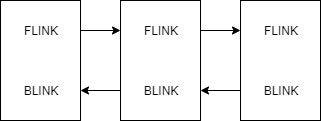
\includegraphics[]{images/eprocess_link.png}
\end{figure}

\begin{figure}[H]
\centering
\caption{EPROCESS linking modified}
\label{fig:dkom}
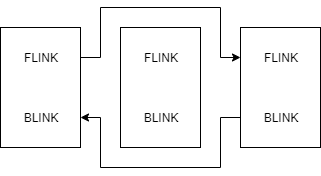
\includegraphics[]{images/dkom.png}
\end{figure}

A process in Windows is composed by threads, for example, a process loading a library will have the library run as a thread. Every thread will have a kernel object inside the non-paged pool to manage called \texttt{\_ETHREAD}. From an \texttt{\_ETHREAD} we can call \texttt{IoThreadToProcess} to get the parent \texttt{\_EPROCESS}, see Listing~\ref{lst:threadtoprocess}. \texttt{\_EPROCESS} has a doubly linked list of \texttt{\_ETHREAD} in \texttt{LIST\_ENTRY ThreadListHead} to list threads of a process.

\begin{lstlisting}[language=c,caption={IoThreadToProcess},label={lst:threadtoprocess}]
PEPROCESS IoThreadToProcess(
  PETHREAD Thread
);
\end{lstlisting}

\subsection[KDBG]{KDBG}

KDBG short for \texttt{Kernel Debugger Block} is one of the commonly used structure when analyzing a memory artifact of Windows. It was created to easy debugging process for developers when writing OS or kernel drivers. As this struture contains pointers to others structures. One pointer contained in KDBG is \texttt{PsActiveProcessHead} which is a pointer to an \texttt{\_EPROCESS}. As previously mentioned, we can walk the list of \texttt{\_EPROCESS} to enumerate all processes.

% TODO: Move this somewhere else

However from Windows 8, this structure is encoded and hinders us from analyzing windows memory. As quoted by the developers of Volatility \cite{kdbgEncoded},

\say{An encoded KDBG can have a hugely negative effect on your ability to perform memory forensics. This structure contains a lot of critical details about the system, including the pointers to the start of the lists of active processes and loaded kernel modules, the address of the PspCid handle table, the ranges for the paged and non-paged pools, etc. If all of these fields are encoded, your day becomes that much more difficult.}

While users of Volatility will suffer a bad day, Rekall's users do not as they use another method without knowledge of KDBG structure \cite{rekallOnKDBGEncoding}. However, KDBG is still an important Windows structure that provides kernel information.

\subsection[Windows dump file]{Windows dump file}

Windows provides a dump file to contains compressed memory data. This file is created by Windows when an error in kernel occur. Third party tools can dump the memory on running machine for example, DumpIt, FTK Imager. This file structure is not documented, however, it was written on Microsoft debug file, Schuster \cite{dmpfile} has written a guide to the file structure. Another dump file type is mini dump file which is documented by Joachim \cite{mdmpfile}. These dump files are commonly used to preserve the system memory state for analysis.

\subsection[Process injection]{Process Injection}
\label{sec:processinjection}

Process injection is a technique to inject a process to another running process. In 2019, Amit Klein and Itzik Kotler gave a talk at US Blackhat conference about the topic \cite{processinjection}. The research is done on Windows 10 x64, they tried to systemize the process injection techniques. Some techniques could still be used although Windows 10 has better security than previous Windows version. A process injected will be more stealthy since the system can only see the parent process. This method is often used by malware to make their process hidden from the system. However, for any process spawn, a thread is always created, so there is always an \texttt{\_ETHREAD} of the process.
